\chapter{How the program works}\label{text:02_program_flow}

% TOC for ch02 {{{
\begin{comment}
	What will be included in this section :
		- Very brief overview :
			- Open the program
			- Load a grid
			- Visualize it
			- Interact with it
			- Save it/close the program
		- Opening the program :
			- What gets created
			- What can you do right now ?
			- What does the code do in the background ?
		- Loading a grid :
			- What can you load ? (filetypes, types of data) -> for types of data, specify more info will be given in technical doc for the new grid api
			- what parameters can you specify ?
			- How to specify them ?
			- What does the code do in the background ?
		- Visualizing a grid :
			- What can you do ? (different viewing modes and how they work, quickly)
			- How do the things get drawn on screen ?
			- How do the different viewers get controlled ?
			- What does the code do in the background ?
		- Interacting with the grids on screen ?
			- What can you do ?
			- How does it work ?
			- What does the code do in the background ?
		- Generating/saving grids
			- What can you do with this ?
			- How does it work ?
			- What options/parameters can you set ?
			- What does the code do in the background ?
\end{comment}
% }}}

% overview of the system {{{
\section{Overview of the system}\label{text:02_program_flow:01_overview}
{
	%		- Visualize it
	%		- Interact with it
	%		- Save it/close the program

	% intro {{{
	As explained beforehand, this program had a few very simple features, all in order to ease the visualization and management of huge datasets. You can load a big 3D image, visualize it in real-time, and interact with it in a very simple fashion. Afterwards, you can save sub-parts of the grid in a new file. There are of course, some limitations to the kinds of images you can load in memory. Most notably, you can only load a few filetypes into the program. Those are \textsc{Tiff} files, \textsc{OME-Tiff} files, and \textsc{Dim/Ima} files.\par
	Let us go through the program as it is supposed to be used, steop by step.\par\myparspace
	% }}}

	% opening program {{{
	\subsubsection*{Opening the program}
	{
		% figure : program ui start {{{
		\begin{figure}[h]
			\label{figure:program_ui_00}
			\centering
			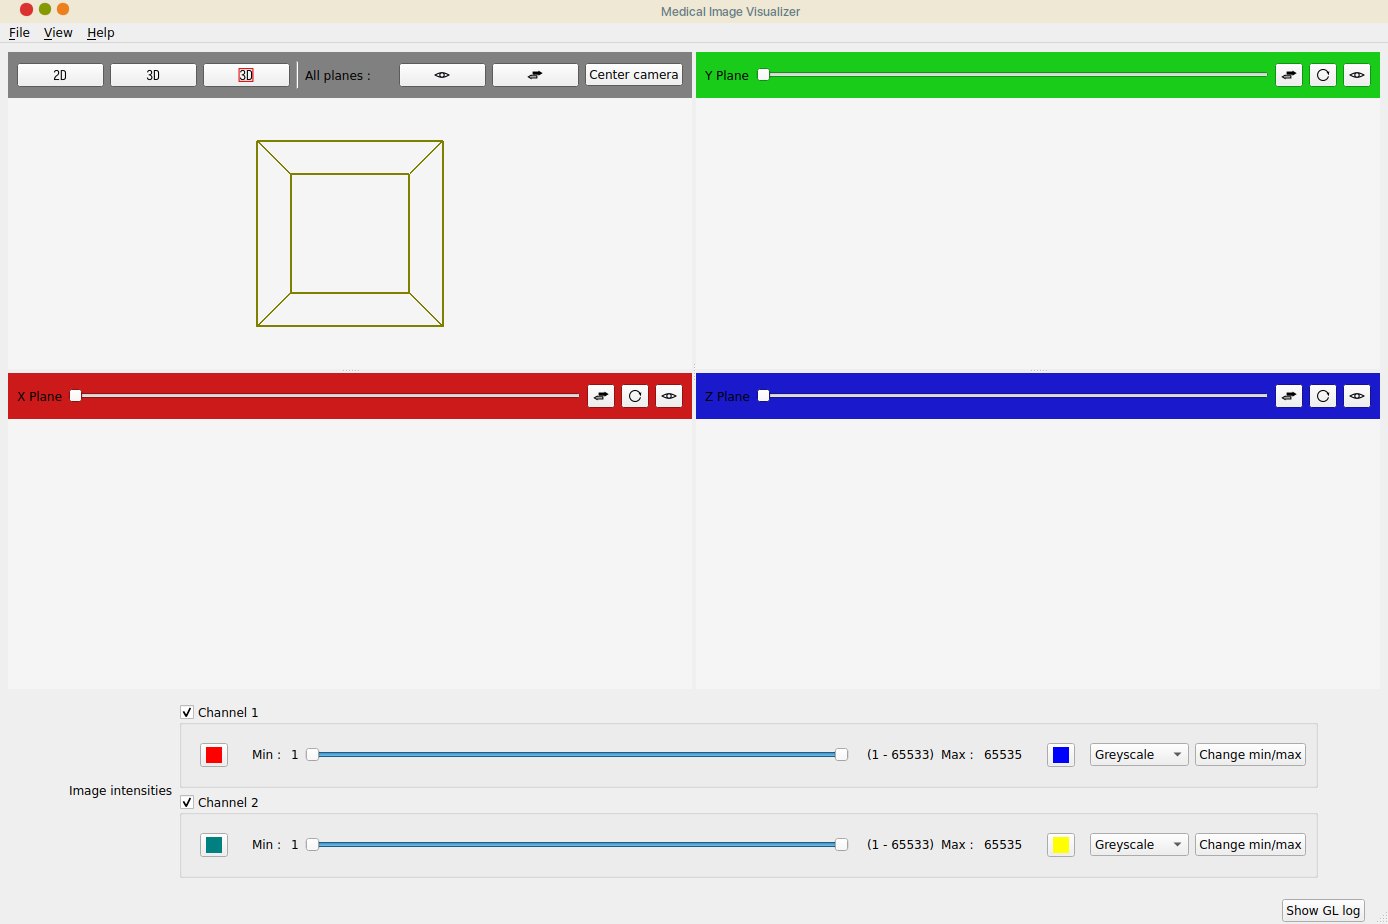
\includegraphics[width=.75\textwidth]{img/program_00.png}
			\caption{The default interface of the program.}
		\end{figure}\par
		% }}}
		% opening : 4 windows & their headers {{{
		Upon opening the program (as illustrated in figure \ref{figure:program_ui_00}), you'll be greeted by four distinct windows directly in the center of the program. The upper left-hand window allows to see the loaded images in three dimensions, and by default only shows an olive-colored wireframe cube. The upper right-hand window will show the contents present at the position of the XZ plane, once an image is loaded. The bottom left-hand and right-hand windows show the contents of the YZ and XY planes respectively, once an image is loaded.\par
		At the top of those four \guillemotleft{}~visualization windows~\guillemotright{}, you'll find a header which can control some of the aspects of the window they're attached to.\par\myparspace
		% }}}
		% bottom : sliders and colors {{{
		The bottom quarter of the program's window contains two group boxes, each containing a range slider (containing two handles), two colored buttons, a drop-down menu and a button labelled \guillemotleft{}~Change min/max~\guillemotright{}. We'll explain what those do in just a moment. And finally, a \guillemotleft{}~Open GL log~\guillemotright{}~ button which is the OpenGL log (intended for debugging).\par
		\myparspace
		% }}}
	}
	% }}}

	% loading a grid {{{
	\subsubsection*{Loading a grid}
	{
	% warning : api in shift {{{
	\textit{Note} : this section of the program contains code that is subject to change, due to an architectural change of the internal grid representation. See section \ref{text:03_software_components:01_image_representation:03_migration} and section \ref{text:03_software_components:01_image_representation:02_modern_grid} for more information.\par\myparspace
	% }}}
	% figure : program file loading dialog {{{
	\begin{figure}[h]
		\centering\label{figure:program_ui_01}
		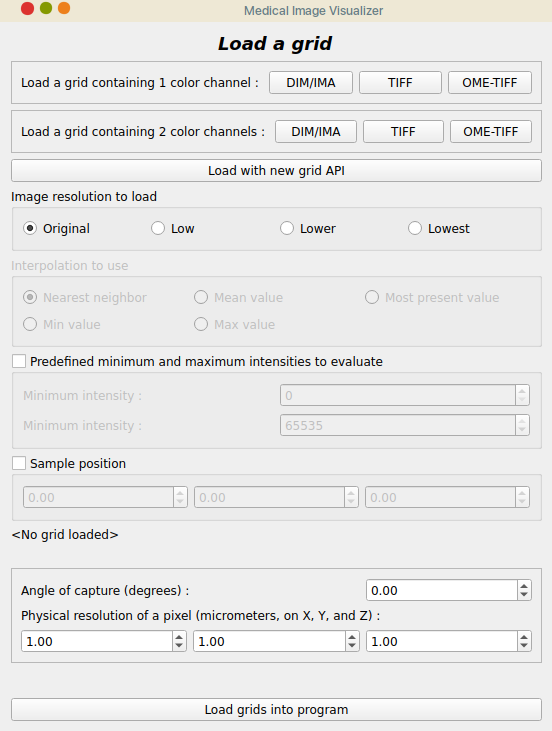
\includegraphics[width=.6\textwidth]{img/program_01.png}
		\caption{Image loading dialog}
	\end{figure}\par
	% }}}
	% intro to loading {{{
	Once the program is open, the user can load a grid by either pressing the \textit{File > Open images} menu item, or by pressing \texttt{\textit{Ctrl+O}}. From there, the user is greeted with a new window, where they can choose the type of file to load.\par
	The different buttons laid out at the top of the window all serve a slightly different purpose. The first group of buttons (in the top frame) allow the user to load a greyscale dataset from disk, using one of the formats available at its disposal. Selecting a filetype and attempting to load another filetype will result in an error and no grid being loaded.
	The next group of buttons tries to load a 2-channel dataset from disk, with the same modalities as before. And the last button is currently only a test of a new implementation of the internal grid representation, and can only load two \guillemotleft{}~stacks~\guillemotright{}~of files saved as \texttt{Tiff}.\par\myparspace
	% }}}
	% list of parameters in the dialog {{{
	Within this window (shown in figure \ref{figure:program_ui_01}), the user can specify a few different parameters. The user-specifiable parameters start from below the \guillemotleft{}~\textit{Load with new grid API}~\guillemotright{}~button. From top to bottom, those are :
	\begin{itemize}
		\item \textit{the resolution to load} : this specifies the amount of downsampling to apply to the image. By default, the grid is loaded in full resolution. And then, the grids are loaded at $\frac{1}{8}$-th, $\frac{1}{64}$-th, or $\frac{1}{512}$-th resolution, by pressing the \textit{Low}, \textit{Lower}, and \textit{Lowest} buttons respectively (each level divides the resolution on each axis by 2).
		\item \textit{the interpolation to apply} : specifies the interpolation to apply when downsampling the grid on load. The user can specify any option amongst \textit{Nearest Neighbor}, \textit{Mean value}, \textit{Most present value}, \textit{Min value}, and \textit{Max value}.
		\item \textit{the range of values to evaluate} : if the user already knows the range of \guillemotleft{}~interesting values~\guillemotright{}~to evaluate, it can be specified here and the visualization pipeline will take it into account when setting the range of values visible.
		\item \textit{sample position} : this allows the user to specify an approximate offset of the dataset from the origin. Completely optional.
		\item \textit{angle of capture} : this parameter is for \textit{di-SPIM} captures that have not yet been resampled in world space. This value (expressed in degrees) will be the angle of capture of the microscope camera from the normal to the sample.
		\item \textit{physical resolution of a pixel} : expressed in micrometers, this will define the size of a voxel in the loaded grid.
	\end{itemize}\par
	% }}}
	% parameters can be left blank, no errors = dimensions in label {{{
	All of those parameters can be specified by the user, or filled automatically if the filetype has additionnal metadata representing those variables. Do note that upon specifying a set of files to load, the window may freeze for a couple of seconds as it parses the stack of filenames. The user will know the grid has been properly parsed without errors if the dimensions of the grid appear in the label in the middle of the window, which currently says \guillemotleft{}~no grid loaded~\guillemotright{}.\par\myparspace
	% }}}
	}
	% }}}

	% visualization & interaction w/ grids {{{
	\subsubsection{Visualizing and interacting with the loaded image}
	{
		After the user specified the grid to load as well as its parameters, the data contained in the grid is processed and uploaded to the GPU. A quick processing step (that might freeze the window) later, and the grid is ready to be visualized.\par
		The controls for the visualization are located at the bottom of the grid, and allow to specify multiple parameters : the range of values to display, as well as the color scale to use.
	}
	% }}}

	% grid generation {{{
	\subsubsection{Generate and save the grid}
	{
		%
	}
	% }}}

}
% }}}

% program flow, object lifetime in the program {{{
\section{Program lifetime}\label{text:02_program_flow:02_object_lifetime}
{
	This section is mainly aimed at developers. It will go through the same program workflow, and detail what resources are created, how they are created and how to find them in the code.

	% opening the program {{{
	\subsubsection{Opening the program}
	{
		%
	}
	% }}}

	% loading grids {{{
	\subsubsection{Loading the grid}
	{
		%
	}
	% }}}

	% visualization / interaction {{{
	\subsubsection{Visualizing and interacting with the loaded image}
	{
		The visualization pipeline is written to be compliant with OpenGL 3.2. This choice was made to ensure a wider portion of the currently-used graphics hardware could run the program. Most notably, the computers at the IGF were not updated to the latest graphics driver (to ensure compatibility with a proprietary software they use), forcing us to downgrade the OpenGL version required to be 3.2.\par
		Most of the program \textit{should} work with OpenGL 2.0, as long as some extensions are required when the program starts (most notably, vertex array objects and buffers should be present). See \textit{Qt}'s and OpenGL's documentation on how to get the available extensions on a system at runtime, and read on to see the technical requirements of the program.

		% should talk about :
		% tetra mesh, range of values init in the scene classes, color scales (that are not in use yet, still
		% uses the ones in the grid !!!), and then the upload of tet mesh to the GPU
	}
	% }}}

	% grid generation {{{
	\subsubsection{Generate and save the grid}
	{
		%
	}
	% }}}
}
% }}}

% Vim modeline, do not touch !
% vim : set breakindentopt=shift\:2 :
